\part{Software Architecture}

Before writing the code for the demos, we started by coming up with an
overall software architecture.  The purpose of this planning was to
write each node so that as other nodes are added to our software
package we do not have to spend time rewriting old code.

This section will describe the decisions we made and what we have
planned.

\section{Node Architecture}

The main document we are basing our software architecture off of is
the following:

\FloatBarrier
\begin{figure}[h]
  \centering
  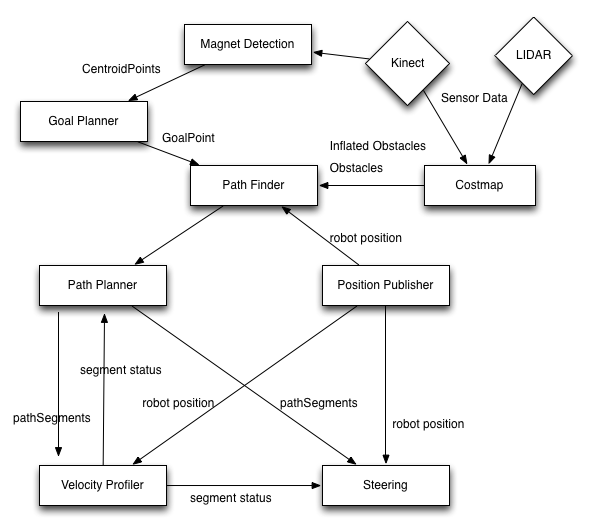
\includegraphics{images/software_architecture.png}
  \caption{Overall software architecture.  Boxes are nodes. Diamonds are sensors.  Arrows denote information being sent between nodes}
  \end{figure}
\FloatBarrier


This figure clearly shows the different nodes we have planned, the
communication message types being passed between them, and areas of
possible future expansion.

The specifications for the nodes in the diagram and the messages being
used will be found in the rest of this section.

\section{ROS Packaging and Stacks}

We have been utilizing ROS stacks to manage our individual ROS packages.
We will try to use a single package per node. This will encourage
appropriate message passing between nodes and make sure they are not too
tightly coupled.

Another benefit is that rosmake will build packages that don't depend
on one another in parallel.  This decreases the build time by a small
amount, which is especially useful when making small changes during testing.

Stacks utilize a \texttt{stack.xml} file which contains dependencies to
be included for every package. The ROS stack will automatically build
all packages within it's root directory.

Complete documentation can be found at 
\url{http://www.ros.org/wiki/Stacks}


\section{Keeping the Nodes in Sync}

Each node runs in its own process which means its possible for the nodes to get out of sync, especially if messages are lost. Lost messages were a problem for us because the nodes do not check if anyone is actually set up to listen to their messages. That meant that if a publishing node started publishing data before the listener the lost messages would cause unexpected behavior in the nodes.

To get around this we added flags to custom message type, such as the new flag. These flags allowed us to continually publish old information until it was no longer valid. The nodes listening to the messages would not consider the information new unless they had no information or the new flag was set. This meant that even if the original message was missed on startup the nodes would eventually get back in sync.

We went with this approach because we were not aware of ROS services at the time we designed the messages and interfaces. ROS services would have allowed us to block until a service became available. It also would have allowed us to get new information on demand. For instance instead of raising an abort flag in segment status when the specified path could not be executed, we could have called a service on the path planner node that computed a new path. This would have saved on bandwidth and made syncing the nodes simpler.

\section{Node Specifications}

To help guide us while writing our nodes we wrote a small
specification for each class seen in the software architecture diagram.

\subsection{Velocity Profiler}
This nodes is responsible for taking in a list of path segments through the PathList and PathSegment message. After receiving the specified path, velocity profiler calculates the optimum trajectory based on the velocity and acceleration constraints in specified in the path segments. In the process of computing the optimum trajectory velocity profiler will blend multiple segments into a single seamless trajectory. After the trajectory is computed velocity profiler is responsible for sending the desired velocity at each point to steering.

\subsubsection{Requirements}
\begin{enumerate}
  \item Velocity Profiler must accept PathList messages
  \item Velocity Profiler must calculate spatial trajectories from
        the accepted PathSegment messages
        \begin{enumerate}
           \item Velocity Profiler must obey all of the path constraints
                 specified in every accepted PathSegment message
        \end {enumerate}
  \item Velocity Profiler must respond to Obstacle messages from Look
        Ahead
        \begin{enumerate}
           \item Velocity Profiler must stop and wait at an obstacle for a
                 specified amount of time
           \item Velocity Profiler must alert Path Planner if an obstacle
                 has not moved after a specified time
        \end{enumerate}
   \item Velocity Profiler must publish a desired velocity based on the computed trajectory
   \item Velocity Profiler must stop when the E-Stop is enabled
   \item Velocity Profiler must resume a plan after the E-Stop is
         disabled
\end{enumerate}
      
\subsection{Look Ahead}

This node enables reactive obstacle detection. As the name implies it is responsible for ``looking'' ahead for obstacles along the path. Currently it uses the LIDAR but using either the costmap or custom code this could be expanded for other sensors such as the Kinect.

  \subsubsection{Requirements}
  \begin{enumerate}
     \item Look Ahead will parse the data from the LIDAR
     \item Look Ahead will detect objects within a minimum of 1 m along the specified path
     \item Look Ahead will exclude obstacle detection of all objects
           outside of the planned path
  \end{enumerate}

\subsection{Steering}
  This node is responsible for correcting the small differences
  between desired and actual heading. It takes in a desired velocity and scales
  its own steering around that value based on the segment type.

  \subsubsection{Requirements}
  \begin{enumerate}
     \item Steering will accept a list of paths
     \item Steering will correct the desired velocities from Velocity
           Profiler
     \item Steering will obey stopping commands in the desired velocity
     \item Steering will stop correcting the path when the E-Stop is pressed.
  \end{enumerate}

\subsection{Path Planner}

This node is responsible for taking in a set of path points and converting it to a list of path segments that form a path through the desired points. It is allowed to throw out conflicting data and select path segment parameters such as the speed.

  \subsubsection{Requirements}
  \begin{enumerate}
    \item Path Planner will receive a list of path points
    \item Path Planner will send out the calculated path in segments
    \item Path Planner will respond to requests for new paths
    \item Path Planner will correct its computed path based on new information in the path point list
  \end{enumerate}

\subsection{Path Finder}

This node is responsible for taking in sensor information and map information and finding a potential points that the robot should navigate to. These points will eventually be constructed into a path segment which will be put together to make an entire path. We implemented multiple instances of this node.

     \subsubsection{Requirments}
     \begin{enumerate}
       \item The path finder will not suggest points in which an obstacle is known to exist
       \item The path finder will return the points in the order in which it suggests navigating to
             them
       \item The path finder will update its suggestion over time as new information is provided
     \end{enumerate}
 
\subsection{Kinect}

This node is responsible for any vision processing and depth map processing that the other nodes need to accomplish their goals.  This includes things such as color detection (based on the image data) and distance detection (based on the depth map). Multiple binaries are included in this node. Each accomplishes different things. The launch file can be customized to launch the ones that are necessary for the task at hand.

  \subsubsection{Requirments}
  \begin{enumerate}
    \item The Kinect node shall receive information from the Microsoft Kinect sensor
    \item The Kinect node shall provide the image processing capabilities to any node that desires it
    \item The Kinect node shall provide depth information to any node that desires it.
  \end{enumerate}

\subsection{Costmap}

This node is responsible for populating the robot's representation of the world map with places it cannot go. It will do so using information from the sensors.

  \subsubsection{Requirments}
  \begin{enumerate}
    \item Costmap shall receive information from the different sensors on the robot
    \item Costmap shall provide a list of points which the robot cannot visit.
  \end{enumerate}
       
\subsection{Goal Planner}

This node is responsible for commanding the movement nodes in order to accomplish useful tasks. This node operates at a higher level from the other nodes and is not concerned with how the robot goes places, only that it goes to the places that goal planner commanded it to go to. Goal planner can receive sensory information in order to determine the places the robot should be going.

  \subsubsection{Requirements}
  \begin{enumerate}
    \item Goal planner shall be capable of determining where the robot should go to accomplish its tasks
    \item Goal planner shall give the movement nodes waypoints to navigate to
  \end{enumerate}

\section{Custom Message Specifications}

\subsection{SegStatus}

Responsible for holding information about the status of a path
segment.  The message format is as follows:

\noindent {\bf uint64 lastSegComplete}\\
\indent Stores the number of the last segment that was fully executed.\\
\\
{\bf uint64 seg\_number}\\
\indent Stores the number identifying the segment the message is
pertaining to.\\
\\
{\bf float64 distance}\\
\indent Stores the distance remaining on a segment.\\

\subsection{Obstacle}

Responsible for holding information about obstacles in the path
segments.  The message format is as follows:

\noindent {\bf bool exists}\\
\indent True when 1 or more obstacles detected in path\\
\indent False when 0 obstacles are detected in path\\
\\
{\bf float64 distance}\\
\indent The distance to the closest obstacle\\

\subsection{BlobDistance}
The Kinect Listener publishes the distance from the center of an image
to the center of a blob.

\noindent {\bf uint32 dist}\\
\indent Distance from the center of the blob to the center of the vision in pixels\\

\subsection{CentroidPoint}
Contains the centroid of the interesting part of an image.

\noindent {\bf bool exists}\\
\indent True when a centroid is found (i.e. image filtering criteria is met)\\
\indent False when no interesting parts are left in the image after filtering\\
\\
\noindent {\bf geometry\_msgs/Point point}\\
\indent The point at which the centroid is.\\

\subsection{Goal}
Incrementally updates the major waypoints the robot is supposed to reach.

\noindent{\bf bool new}\\
\indent True when a new goal is published.\\
\\
\noindent{\bf bool none}\\
\indent Set to true when the robot should not change its present location.\\
\\
\noindent{\bf geometry\_msgs/Point goal}\\
\indent The coordinates of the desired goal\\

\subsection{PathList}
A list of path segments that make up a path.

\noindent {\bf msg\_alpha/PathSegment[] segments}\\
\indent The path segment specifications that the robot must follow, in the order they must be followed.\\

\subsection{PathSegment}
Path Segments that are generated by the Path Planner node.

\noindent {\bf int8 seg\_type}\\
\indent The segment type can be a line, arc, or spin, 1,2 or 3 respectively.\\
\\
\noindent {\bf bool relative}\\
\indent Set to true when the path is in the robot's coordinate frame.\\
\indent Set to false when the path is in the map's coordinate frame.\\
\\
\noindent{\bf float64 seg\_length}\\
\indent The length of a path segment.\\
\\
\noindent{\bf geometry\_msgs/Point ref\_point}\\
\indent The reference point of a path segment.\\
\\
\noindent{\bf geometry\_msgs/Quaternion init\_tan\_angle}\\
\indent The initial tangent angle of a path segment.\\
\\
\noindent{\bf float64 curvature}\\
\indent The curvature of a path segment.\\
\\
\noindent{\bf geometry\_msgs/Twist max\_speeds}\\
\indent Maximum speed for a path segment.\\
\\
\noindent{\bf geometry\_msgs/Twist min\_speeds}\\
\indent Minimum speed for a path segment.\\
\\
\noindent{\bf float64 accel\_limit}\\
\indent Acceleration limit for a path segment \\
\\
\noindent{\bf float64 decel\_limit}\\
\indent Deceleration limit for this segment.\\

\subsection{PointList}
Points that the robot should be steering to.

\noindent{\bf bool new}\\
\indent Set to true if points in the message have changed\\

\noindent{\bf geometry\_msgs/Point[] points}\\
\indent Contains the list of points in the order they are supposed to be used in\\

\section{Topics}

\subsection{des\_vel}
Velocity Profiler publishes the desired velocity based on the robot's
current point in space the current and next path segments.  This
velocity is then corrected by steering.

\subsection{cmd\_vel}
Steering publishes the final velocity to the robot's motors.  The
final velocity is a corrected version of the velocity in the des\_vel topic.

\subsection{base\_laser1\_scan and base\_scan}
base\_laser1\_scan is used on the robot\\
base\_scan is used in the simulator\\

\noindent Used to send out LIDAR data from the cRIO.

\subsection{seg\_status}
Velocity profiler publishes the status of what part of the desired path it is executing.  Nodes such as steering subscribe to it.

\subsection{path}
Path Publisher publishes the planned path segments in a PathList message to this topic.  The
published segments are used by steering, velocity\_profiler and other nodes.

\subsection{point\_list}
The path finder node publishes a list of points for the pathplanner to generate path segments from.

\subsection{goal\_point}
The goal publisher sends a goal to the path finder node that determines the end point of the desired points list.

\subsection{obstacles}
Look ahead publishes whether or not there is an obstacle within the bounded box area directly in front of the robot.

\subsection{motors\_enabled}
Estop publishes whether or not the estop is off.

\subsection{map\_pos}
Publishes the current location of the robot in map space. This prevents all of nodes from having to do the odom to map transformation. It also allows us to rostopic echo the topic to easily verify that the robot knows its own position.